\documentclass{beamer}
\usetheme{Warsaw}
\setbeamertemplate{headline}{}

\usepackage{ae,lmodern}
\usepackage[english]{babel}
\usepackage[utf8]{inputenc}
\usepackage[T1]{fontenc}

\usepackage{caption}
\captionsetup[figure]{labelformat=empty}

\PassOptionsToPackage{usenames,dvipsnames}{xcolor}
\usepackage{xcolor,colortbl}
\definecolor{DarkGrey}{HTML}{222222}
\definecolor{DarkBlue}{HTML}{004BA9}
\definecolor{DarkRed}{HTML}{CC1111}
\definecolor{DarkGreen}{HTML}{117711}
\definecolor{DarkOrange}{HTML}{CC7000}
\definecolor{LightGrey}{HTML}{DDDDDD}
\definecolor{LightBlue}{HTML}{F0F8FF}
\definecolor{codegreen}{rgb}{0,0.6,0}
\definecolor{codepurple}{rgb}{0.58,0,0.82}

\usepackage[cache=false]{minted}
\setminted[bash]{
   bgcolor=LightBlue,
   breaklines, breakanywhere,
   frame=single,
   autogobble
}
\usemintedstyle[python]{native}
\setminted[python]{
   bgcolor=black,
   breaklines, breakanywhere,
   autogobble
}

\usepackage{listings}
\usepackage{lstautogobble}
\lstdefinestyle{bash}{
    backgroundcolor=\color{DarkGrey},   
    commentstyle=\color{codegreen},
    keywordstyle=\color{magenta},
    numberstyle=\tiny\color{DarkGrey},
    stringstyle=\color{codepurple},
    basicstyle=\ttfamily\tiny\color{LightGrey},
    escapeinside={\%*}{*)},
    breakatwhitespace=false,         
    breaklines=true,                 
    captionpos=b,                    
    keepspaces=true,                 
    numbers=left,                    
    numbersep=5pt,                  
    showspaces=false,                
    showstringspaces=false,
    showtabs=false,
    showlines=false,
    tabsize=2
}

\usepackage{tikz}
\usetikzlibrary{calc,decorations.pathreplacing,arrows,arrows.meta,shapes,patterns, positioning}
\newcommand\BigLength{14.6em}
\newcommand\Height{2em}
\newcommand\Sep{0.6em}
\newcommand\Center{\BigLength*1/2}
\newcommand\BigBox{\BigLength+\Sep}
\newcommand\HalfBox{\BigLength*1/2-\Sep*1/4}
\newcommand\HalfLength{\BigLength*1/2-\Sep*5/4}
\newcommand\CenterL{\BigLength*1/4-\Sep*1/8}
\newcommand\CenterR{\BigLength*3/4+\Sep*1/8}
\tikzstyle{layer}=[rectangle,thick,text centered,
                     minimum height=\Height,minimum width=\BigLength]
\tikzstyle{short}=[rectangle,thick,text centered,
                     minimum height=\Height,minimum width=\HalfLength]
\tikzstyle{dibox}=[rectangle,thick,semitransparent,
                     minimum height=(\Height+\Sep)*2,minimum width=\BigBox]
\tikzstyle{vmbox}=[rectangle,thick,semitransparent,
                     minimum height=(\Height+\Sep)*3,minimum width=\HalfBox]
\tikzstyle{ctbox}=[rectangle,thick,semitransparent,
                     minimum height=(\Height+\Sep)*2,minimum width=\HalfBox]
\tikzstyle{vebox}=[rectangle,thick,semitransparent,
                     minimum height=(\Height+\Sep)*1,minimum width=\HalfBox]

\usepackage{hyperref}
\usepackage{grffile}


\AtBeginSection[]
{
   \begin{frame}
      \tableofcontents[currentsection]
   \end{frame}
}

\AtBeginSubsection[]
{
   \begin{frame}
      \tableofcontents[currentsection, currentsubsection, sectionstyle=shaded]
   \end{frame}
}

%----------------------------------------------------------------------------------------
\title{Introduction to Data Science}
\subtitle{with Python}
%----------------------------------------------------------------------------------------
\author{Alexis Bogroff}
\date{\today}


\begin{document}

\begin{frame}
   \titlepage
\end{frame}

\begin{frame}\frametitle{Presenter}
   \begin{minipage}{0.3\linewidth}
      \centering
      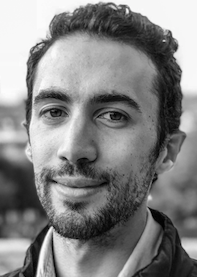
\includegraphics[width=0.6\textwidth]{../images/AlexisBogroff.png} \\
   \end{minipage}
   \begin{minipage}{0.6\linewidth}
      \noindent Alexis Bogroff \\
      Lecturer and Mentor in Data Science \\
      at Paris 1 Panthéon-Sorbonne, ESILV, Openclassrooms, EM-Lyon
   \end{minipage}
   \\[2ex]
   \visible<2->{\begin{itemize}
      \item 4 years Teaching Assistant and lecturer in VBA, Python for finance, SQL, Data Analysis and Data Science
      \item 9 months Researcher Assistant at Paris 1 Panthéon-Sorbonne within H2020 European Project
      \item 1 year Data Scientist at Pléiade Asset Management
   \end{itemize}}
   \hfill
\end{frame}

% \begin{frame}\frametitle{Overview}
%    \Large
%    \centering
%    Financial Engineering with Python Linux and Git \\[2ex]
%    \begin{minipage}{0.32\linewidth}
%       \includegraphics[width=0.8\textwidth]{../images/linux-1-logo-svg-vector.pdf}
%    \end{minipage}
%    \begin{minipage}{0.32\linewidth}
%       \includegraphics[width=0.8\textwidth]{../images/Git-logo.pdf}
%    \end{minipage}
%    \begin{minipage}{0.32\linewidth}
%       \includegraphics[width=0.9\textwidth]{../images/Python_logo_and_wordmark.pdf}
%    \end{minipage}
%    \pause
%    \\[3ex]
%    Free and everywhere stack \\
%    To find a job and be operational
% \end{frame}

% \begin{frame}\frametitle{Lecture Organisation}
%    \begin{itemize}[<+->]
%       \item Prerequisite:
%       \begin{enumerate}
%          \item Have a Linux environment working on your personal computer
%          \item[] (it can be WSL2 on Windows, Amazon EC2 for a distant solution)
%          \item Install Git
%          \item Install Python
%       \end{enumerate}
%       \vspace{2em}
%       \item Exam:
%       \begin{itemize}
%          \item Last QCM 1/2
%          \item Project 1/2
%       \end{itemize}
%    \end{itemize}
% \end{frame}


\begin{frame}
   \tableofcontents
\end{frame}

% =============================================================================
% =============================================================================
\section{Predictions}
% 3 Hours course
% =============================================================================
% =============================================================================


%------------------------------------------------------------------------------
\subsection{Predictions: What does that mean?}
%------------------------------------------------------------------------------
% Use cases

\begin{frame}\frametitle{Predictions: What does that mean?}
   What is modeled?
   \vspace{.3cm}
   \begin{itemize}
      \item Continuity (stationarity)
      \item Correlation (pattern)
   \end{itemize}
   \begin{minipage}{0.60\linewidth}
      \begin{figure}[H]
         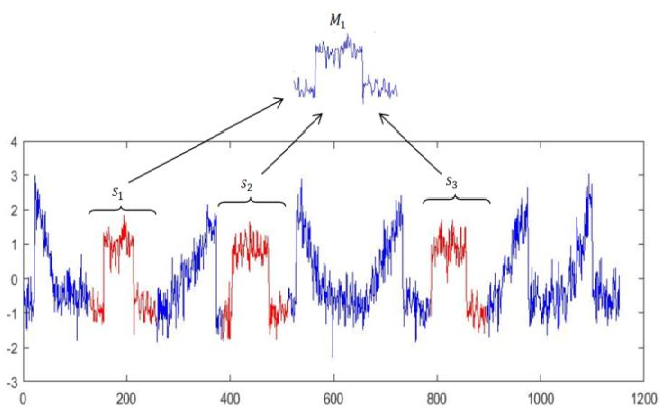
\includegraphics[scale=.4]{../images/illustrations/model_pattern.png}
      \end{figure}
   \end{minipage}
\end{frame}


\begin{frame}\frametitle{Predictions: What does that mean?}
   What is modeled?
   \vspace{.5cm}
   \begin{itemize}
      \item Correlation vs Causality\footnote{\href{Spurious correlations site}{https://www.tylervigen.com/spurious-correlations}}
   \end{itemize}
   \begin{minipage}{0.60\linewidth}
      \begin{figure}[H]
         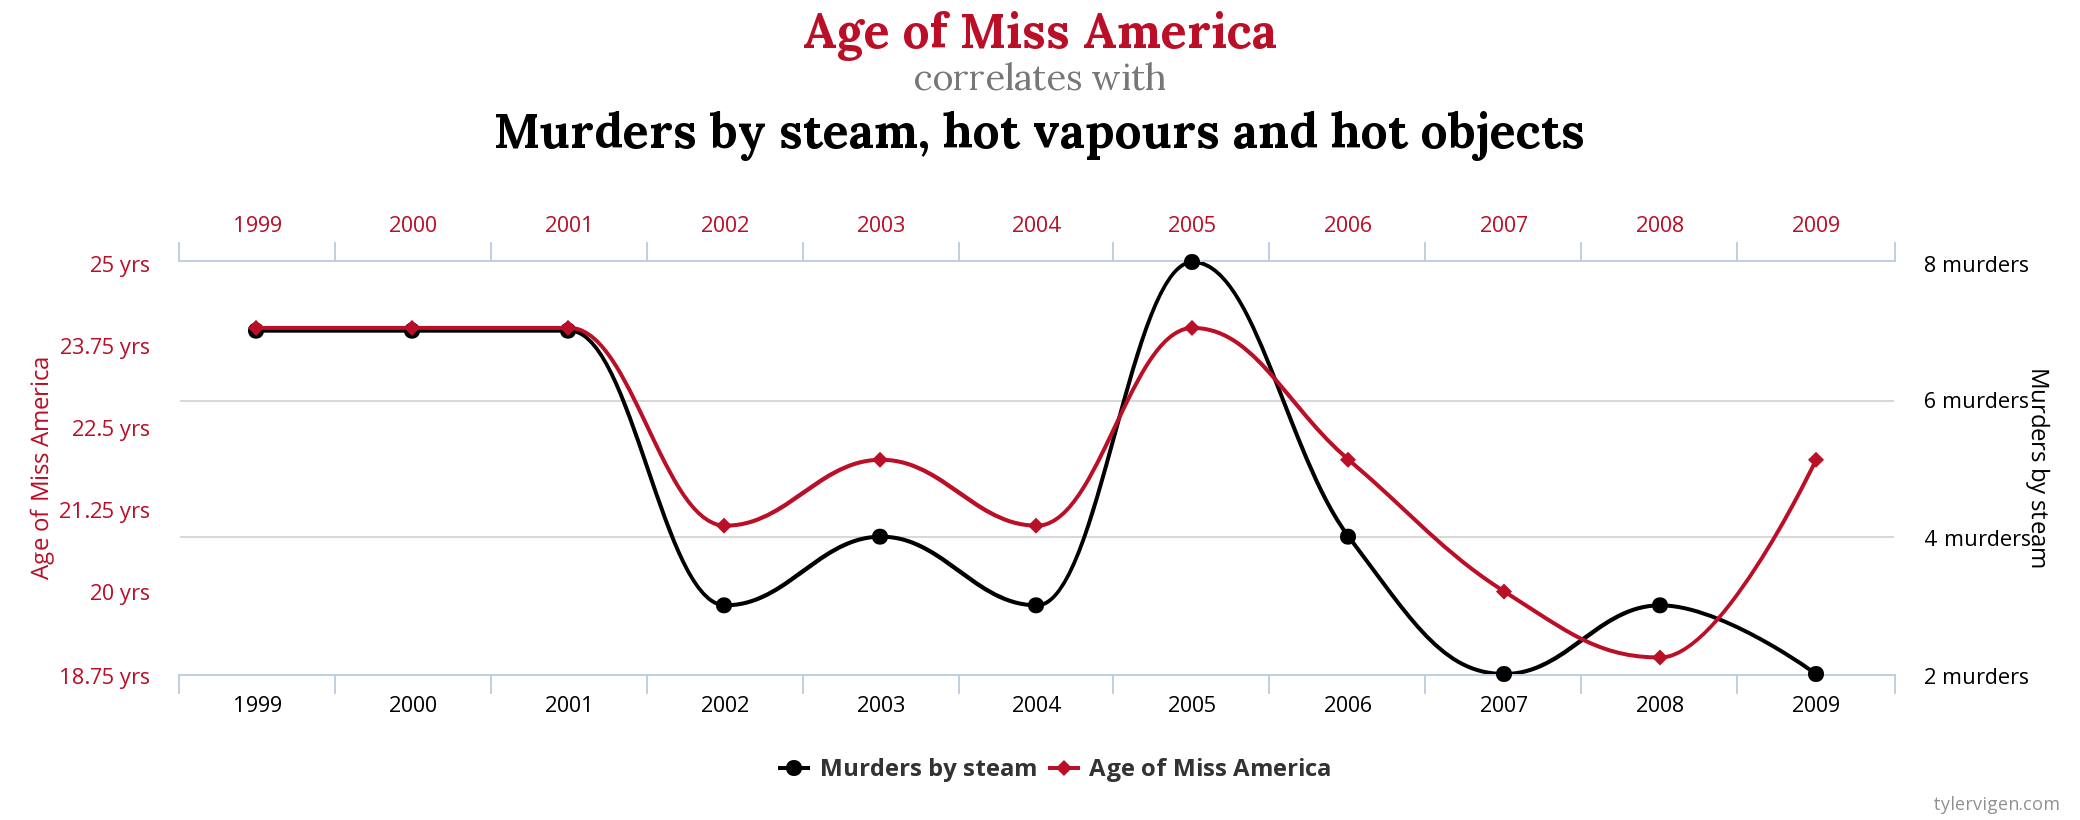
\includegraphics[scale=.15]{../images/illustrations/model_spurious_correlation.png}
      \end{figure}
   \end{minipage}
\end{frame}


\begin{frame}\frametitle{Predictions: Examples}
   \begin{itemize}
      \item Present:
      \begin{itemize}
         \item Electricity consumption based on other cities (e.g. Seattle)
         \item Missing values (interpolation, extrapolation)
         \item Client category
         \begin{minipage}{0.6\linewidth}
            \begin{figure}[H]
               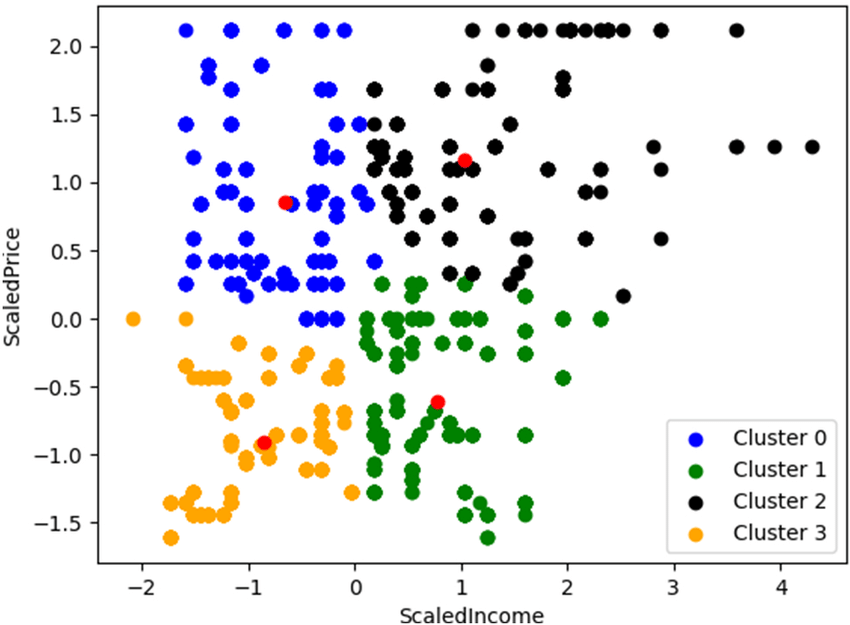
\includegraphics[scale=.1]{../images/illustrations/model_client.png}
            \end{figure}
         \end{minipage}
      \end{itemize}
      \item Future:
      \begin{itemize}
         \item Electricity consumption next month (time series)
         \begin{minipage}{0.60\linewidth}
            \begin{figure}[H]
               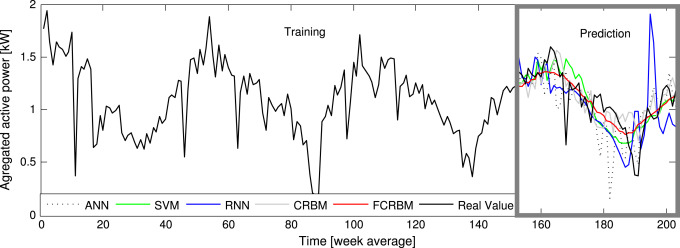
\includegraphics[scale=.35]{../images/illustrations/model_electricity.jpg}
            \end{figure}
         \end{minipage}
         \item Client clicking add (recommander sys.)
         \item Pedestrian and cars trajectories (RL)
      \end{itemize}
   \end{itemize}
   % TODO: add graph with predictions
\end{frame}


%------------------------------------------------------------------------------
\subsection{Supervised ML}
%------------------------------------------------------------------------------

\subsubsection{Regression}


\begin{frame}\frametitle{Regression}
   \begin{itemize}
      \item Linear regression
      \item Simple: $Y = aX + b$
      \item Multiple: $Y = a_1X_1 + a_2X_2 + \dots + a_nX_n + b$
   \end{itemize}

   \begin{figure}[H]
      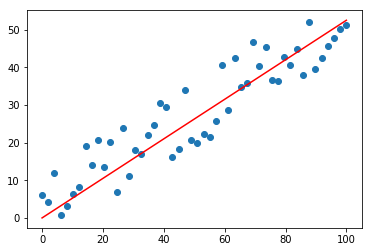
\includegraphics[scale=.35]{../images/illustrations/model_linear_regression.png}
   \end{figure}
\end{frame}


\begin{frame}\frametitle{Regression}
   \begin{itemize}
      \item Polynomial regression
      \item Simple: $Y = a_1X + a_2X^2 + \dots + a_nX^n +b$
      \item Multiple: $$Y = a_{11}X_1 + a_{21}X_2 + a_{n1}X_n + a_{12}X_1^2 + a_{22}X_2^2 + a_{n2}X_n^2 + $$
                           $$\dots + a_{1m}X_1^m + a_{2m}X_2^m + a_{nm}X_n^m + b$$
   \end{itemize}
   \begin{figure}[H]
      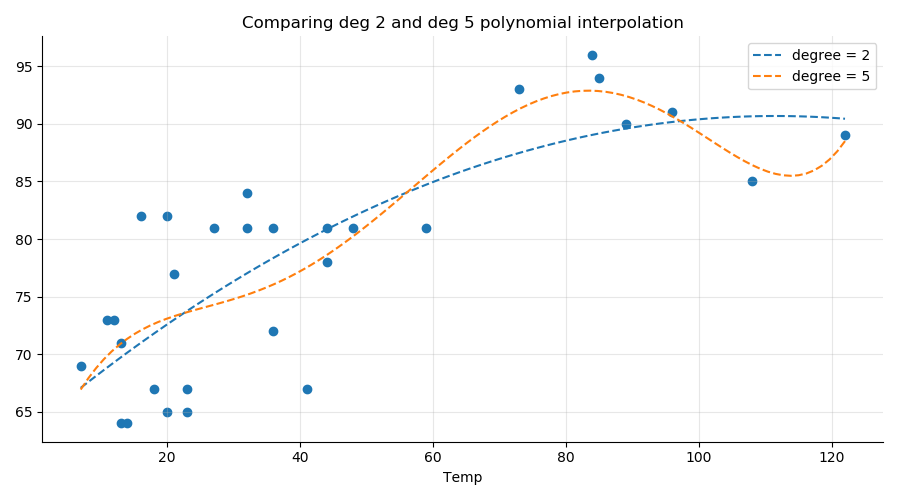
\includegraphics[scale=.35]{../images/illustrations/model_polynomial_regression.png}
   \end{figure}
\end{frame}


\begin{frame}\frametitle{Regression}
   \begin{itemize}
      \item Fight multicolinearity
      \begin{itemize}
         \item Ridge: lower weights
         \item Lasso: set weights to zero
         \item Elastic Net: combine both
      \end{itemize}
   \end{itemize}
   \begin{figure}[H]
      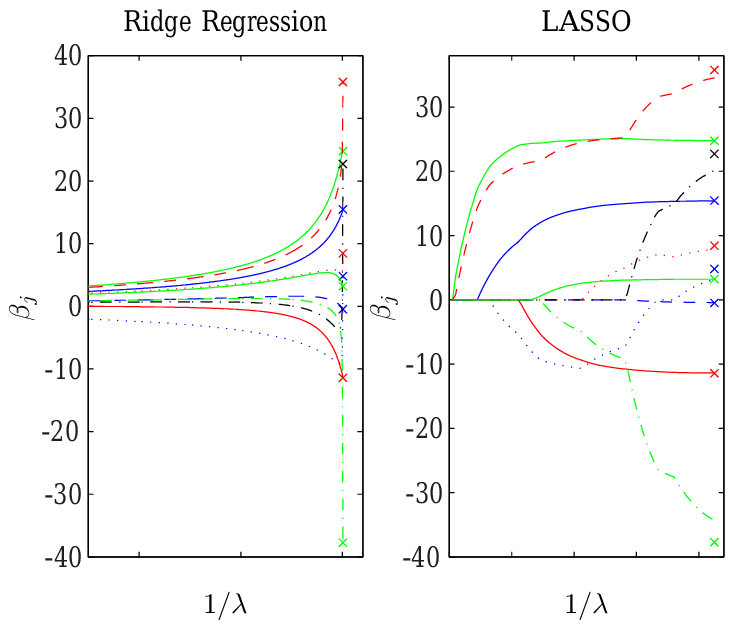
\includegraphics[scale=.23]{../images/illustrations/model_ridge_lasso.png}
   \end{figure}
\end{frame}


\begin{frame}\frametitle{Regression}
   \begin{itemize}
      \item SARIMA: seasonal, auto-regressive, integrated, moving average
      \item Parametric model that capture patterns like:
      \begin{itemize}
         \item Trend
         \item Cycle
         \item Season
      \end{itemize}
   \end{itemize}
\end{frame}


\begin{frame}\frametitle{Regression}
   \begin{itemize}
      \item Deep Learning (RNN, LSTM)
   \end{itemize}
   \begin{figure}[H]
      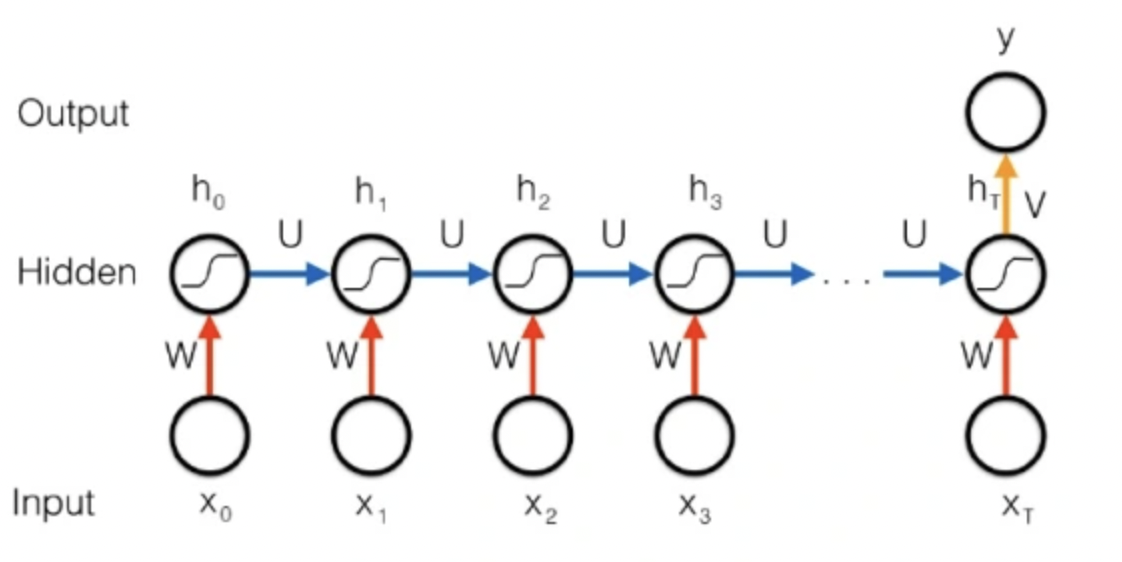
\includegraphics[scale=.35]{../images/illustrations/model_rnn.png}
   \end{figure}
   \begin{figure}[H]
      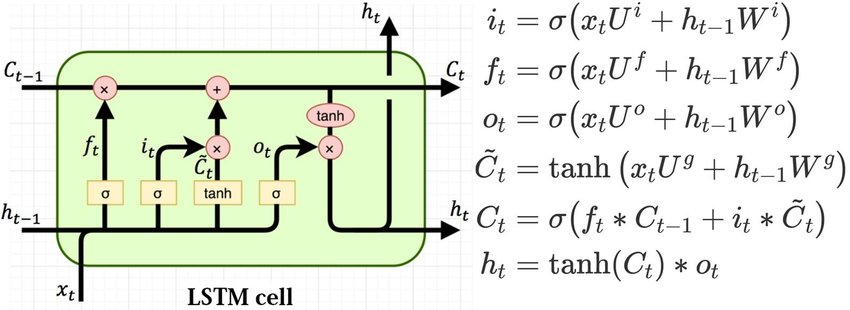
\includegraphics[scale=.35]{../images/illustrations/model_lstm.png}
   \end{figure}
\end{frame}


\subsubsection{Classification}

\begin{frame}\frametitle{Classification}
   \begin{itemize}
      \item Logistic regression
      $\frac{1}{1 + e^{-z}}$ with \textit{z} linear (polynomial) regression
      \begin{figure}[H]
         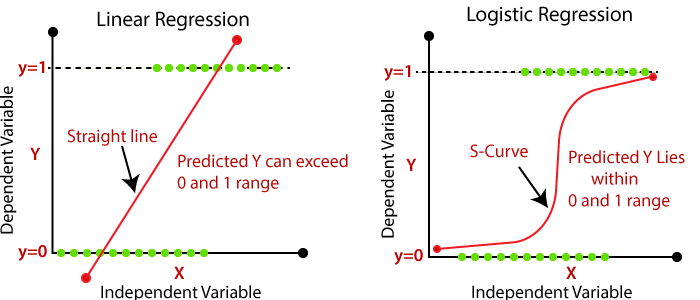
\includegraphics[scale=.35]{../images/illustrations/model_logistic_regression.png}
      \end{figure}
      \begin{figure}[H]
         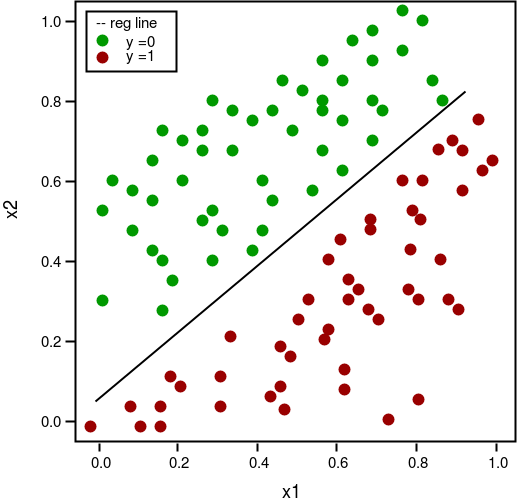
\includegraphics[scale=.2]{../images/illustrations/model_logistic_regression_example.png}
      \end{figure}
   \end{itemize}
\end{frame}


\begin{frame}\frametitle{Classification}
   \begin{itemize}
      \item Tree (ensemble models, RF, XGBoost)
      \begin{figure}[H]
         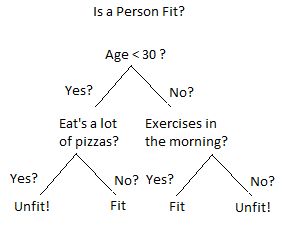
\includegraphics[scale=.35]{../images/illustrations/model_tree.png}
      \end{figure}
      \begin{figure}[H]
         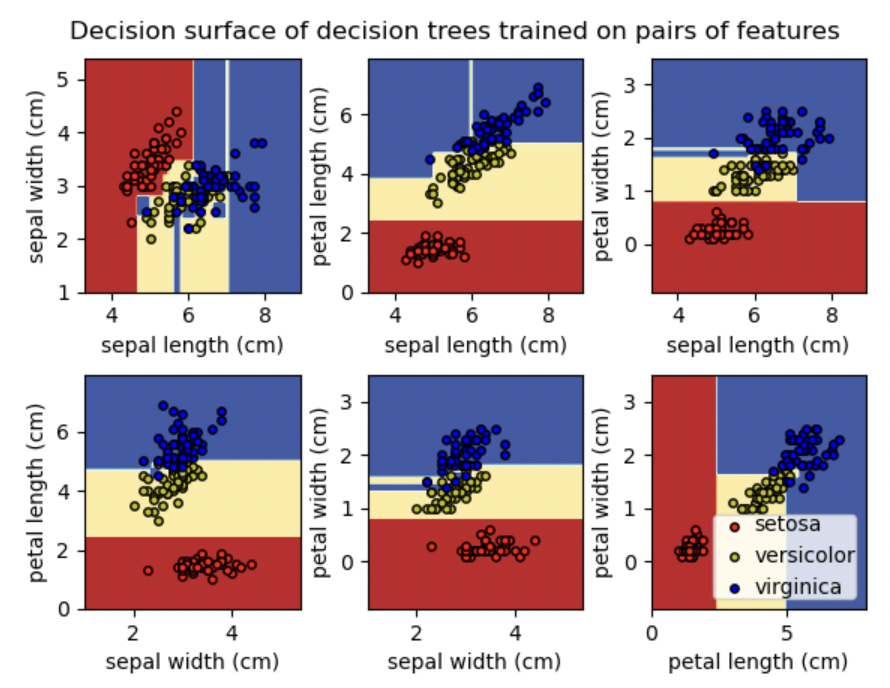
\includegraphics[scale=.35]{../images/illustrations/model_tree_example.png}
      \end{figure}
   \end{itemize}
\end{frame}



\begin{frame}\frametitle{Classification}
   \begin{itemize}
      \item K-means
      \begin{itemize}
         \item Positionnement
      \end{itemize}
      \begin{enumerate}
         \item Capture (iter 1)
         \item Recentrage (iter 2)
      \end{enumerate}
      \begin{figure}[H]
         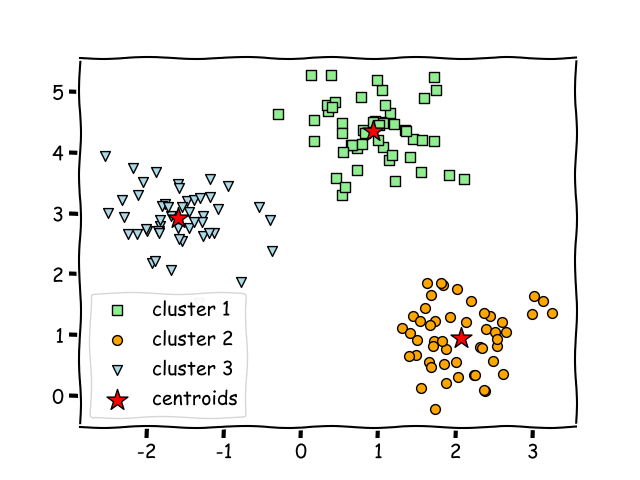
\includegraphics[scale=.35]{../images/illustrations/model_kmeans.png}
      \end{figure}
   \end{itemize}
\end{frame}


\begin{frame}\frametitle{Classification}
   \begin{itemize}
      \item Neural Network (Deep Learning: CNN)\footnote{\href{https://playground.tensorflow.org/}{https://playground.tensorflow.org/}}
      \begin{figure}[H]
         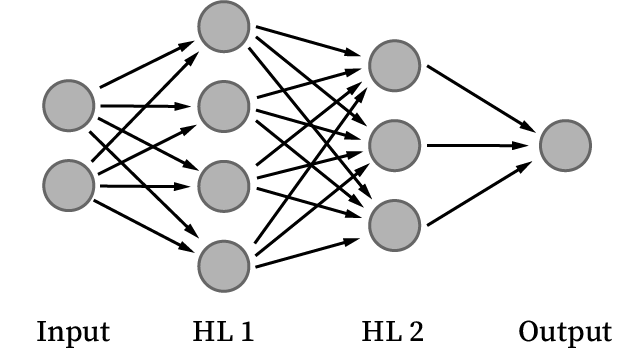
\includegraphics[scale=.25]{../images/illustrations/model_neural_network.png}
      \end{figure}
      
      \item Gradient descent
      \begin{figure}[H]
         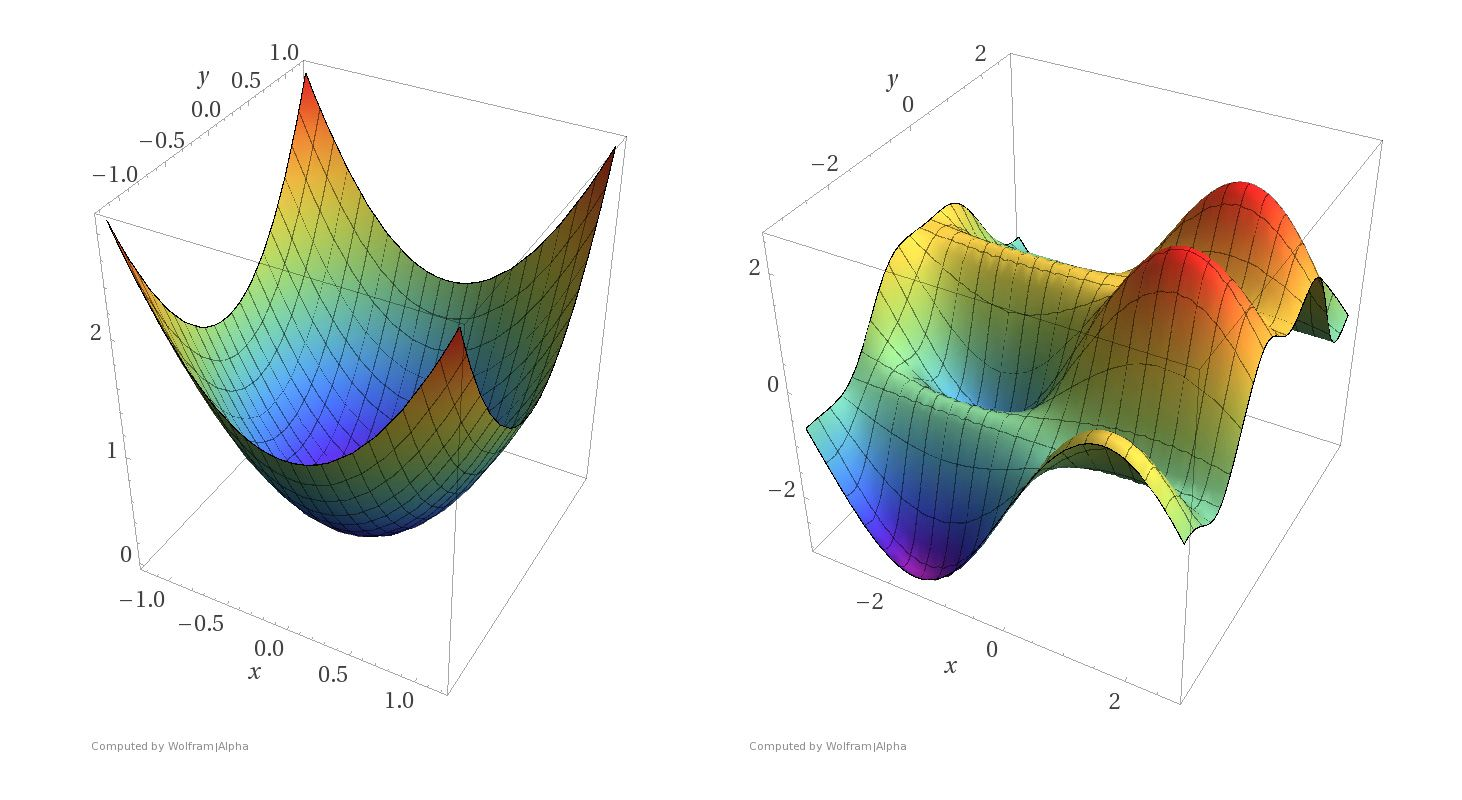
\includegraphics[scale=.15]{../images/illustrations/model_optimization_gradient_descent.jpeg}
      \end{figure}
   \end{itemize}
\end{frame}


%------------------------------------------------------------------------------
\subsection{Unsupervised ML}
%------------------------------------------------------------------------------

\begin{frame}\frametitle{Unsupervised ML}
   \begin{itemize}
      \item Tasks
      \begin{itemize}
         \item Clustering (grouping)
         \item Dimensionality reduction
      \end{itemize}
   \end{itemize}
   \begin{figure}[H]
      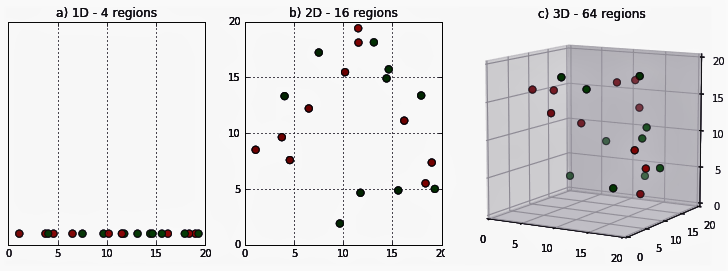
\includegraphics[scale=.35]{../images/illustrations/model_dimension_reduction.png}
   \end{figure}
\end{frame}


\begin{frame}\frametitle{Unsupervised ML}
   \begin{itemize}
      \item Models
      \begin{itemize}
         \item Knn: entropy minimisation principle\\
         (min var intraclass, max var interclass)
         \item Hierarchical Clustering (dendrogram)
      \end{itemize}
   \end{itemize}
   \begin{figure}[H]
      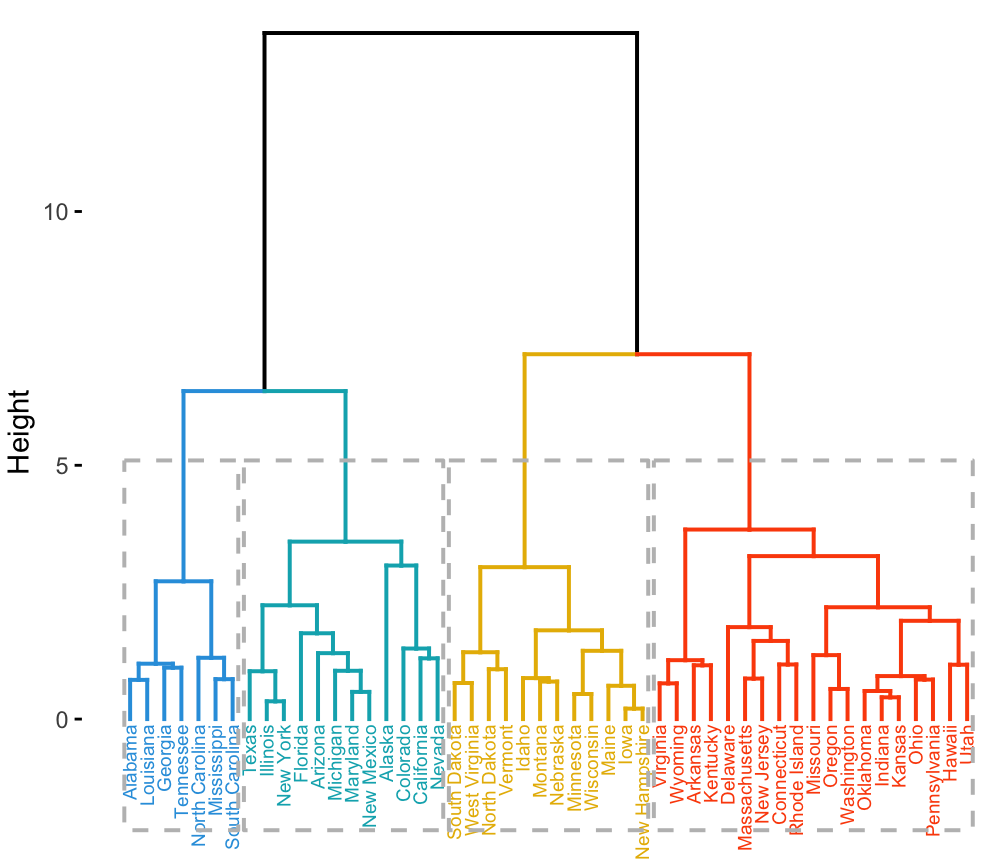
\includegraphics[scale=.18]{../images/illustrations/model_hierarchical_clustering.png}
   \end{figure}

\end{frame}


\begin{frame}\frametitle{Unsupervised ML}
   \begin{itemize}
      \item Models
      \begin{itemize}
         \item PCA
      \end{itemize}
   \end{itemize}
   \begin{figure}[H]
      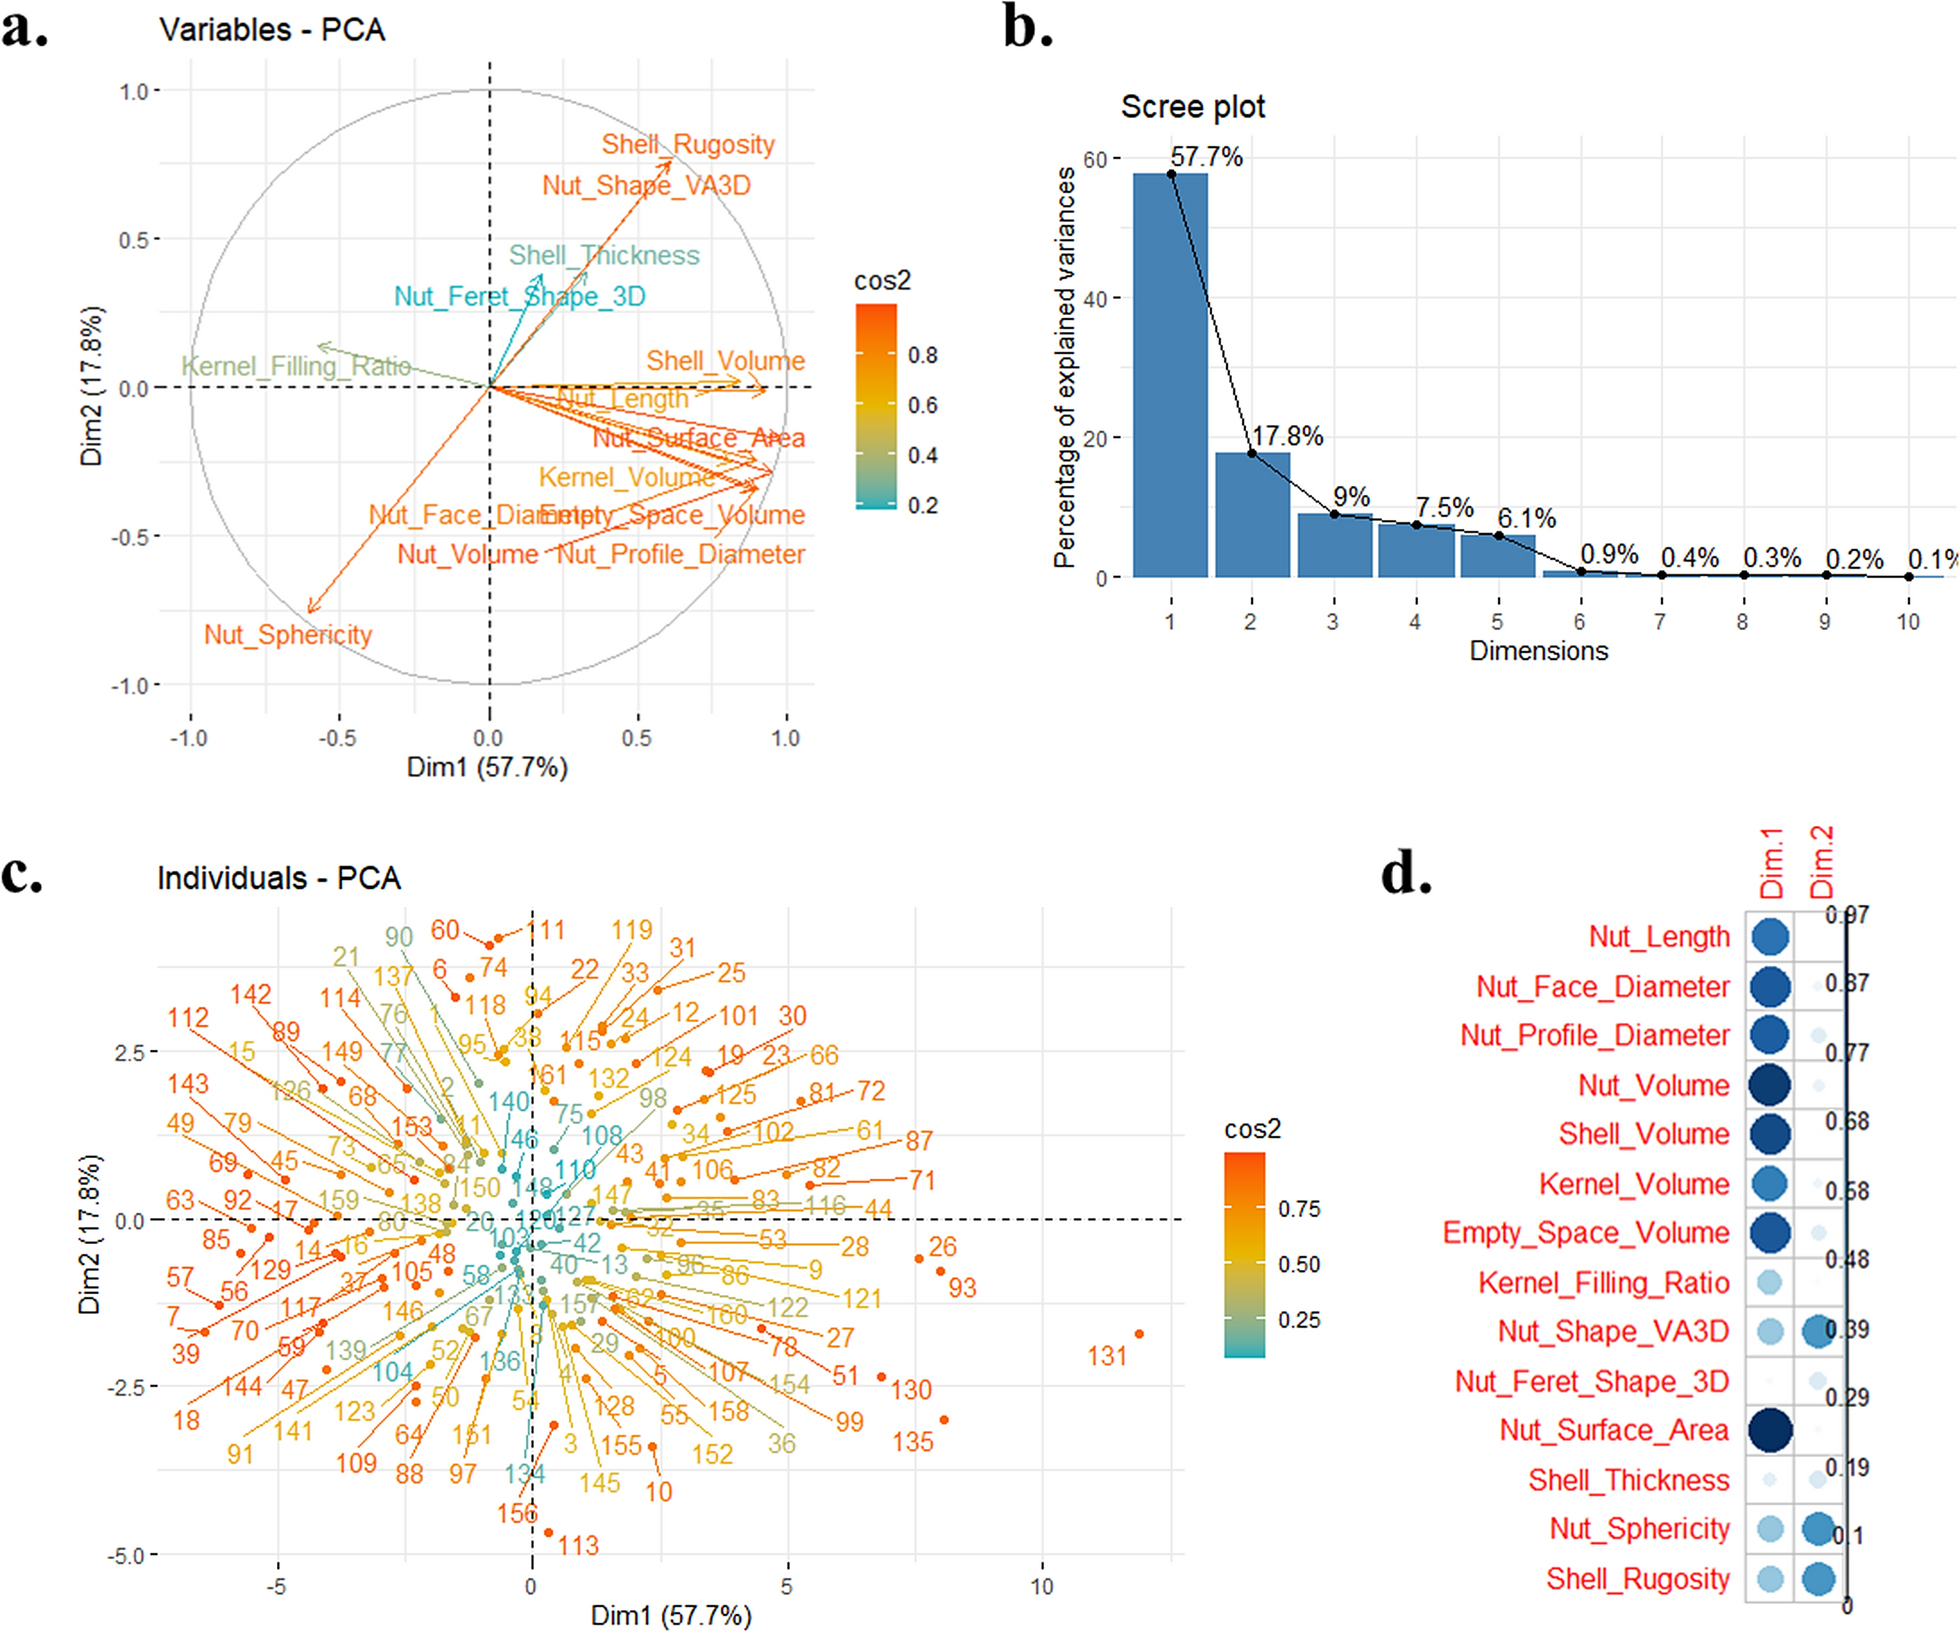
\includegraphics[scale=.13]{../images/illustrations/model_pca_graphs.png}
   \end{figure}
\end{frame}




%------------------------------------------------------------------------------
\subsection{Optimizing models}
%------------------------------------------------------------------------------

\begin{frame}\frametitle{Optimizing models - Control fit}
   \begin{itemize}
      \item Objective: generalization, i.e. good performance on out-of-sample data
      \item Control over/under-fitting
   \end{itemize}
   \begin{figure}[H]
      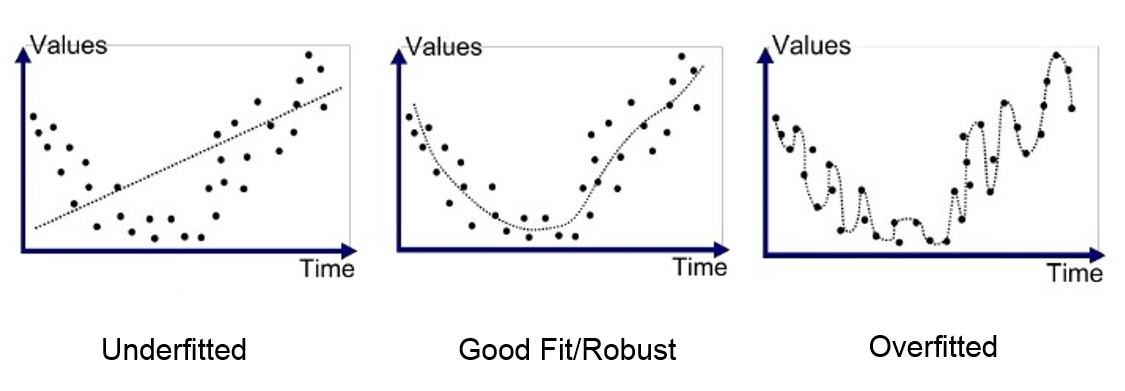
\includegraphics[scale=.25]{../images/illustrations/model_fit.png}
   \end{figure}
\end{frame}

\begin{frame}\frametitle{Optimizing models - Control fit}
   \begin{itemize}
      \item Parameters
      \item Hyperparameters
      \item Train, cross-validate, test
   \end{itemize}
   \begin{figure}[H]
      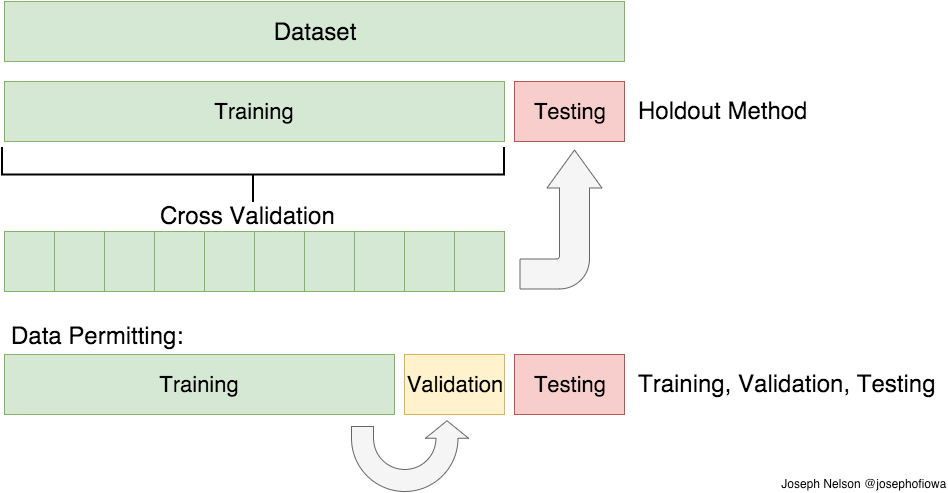
\includegraphics[scale=.25]{../images/illustrations/model_split_data.png}
   \end{figure}
\end{frame}

\begin{frame}\frametitle{Optimizing models - Control fit}
   \begin{itemize}
      \item Feature importance
   \end{itemize}
   \begin{figure}[H]
      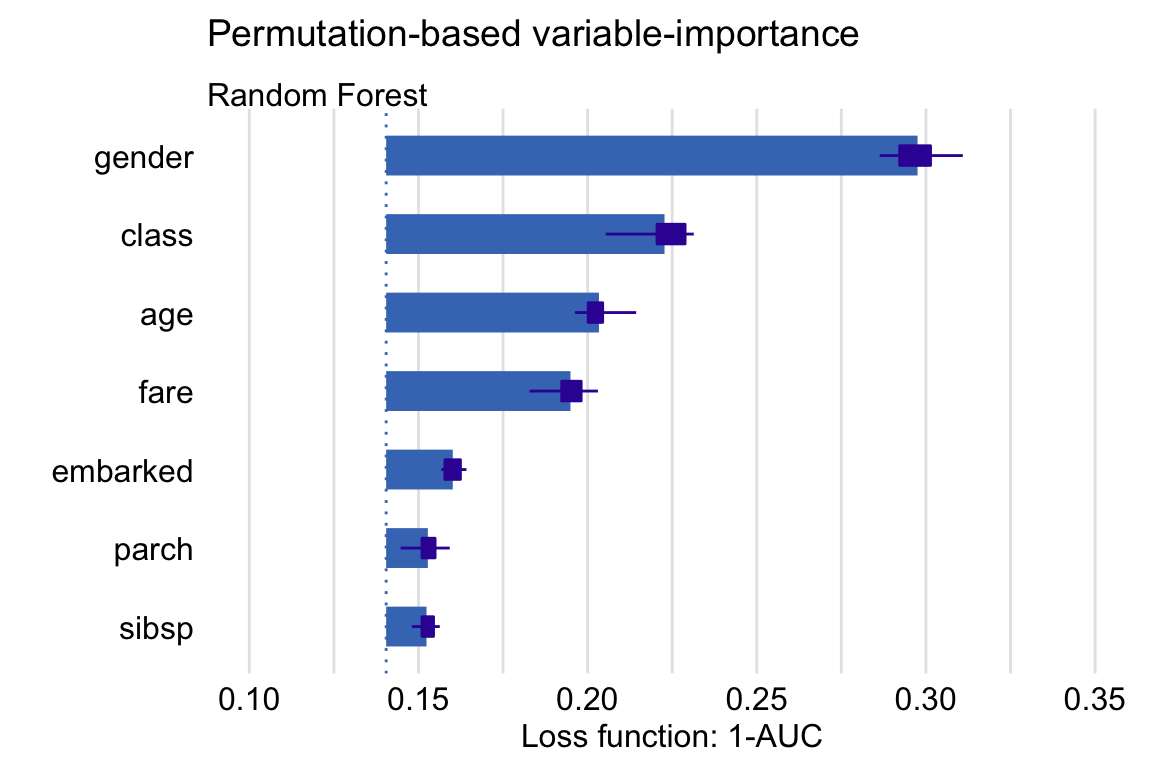
\includegraphics[scale=.25]{../images/illustrations/model_feature_importance.png}
   \end{figure}
\end{frame}



\begin{frame}\frametitle{Optimizing models - Issues}
   \begin{itemize}
      \item Multicolinearity
      \item Data Leakage: data not available at prediction time
      \item Unbalanced Datasets (weights on cost function, SMOTE, Auto-encoder)
   \end{itemize}
\end{frame}


\begin{frame}\frametitle{Metrics}
   \begin{itemize}
      \item Regression
      \begin{itemize}
         \item RMSE
         \item $R^2$
      \end{itemize}

      \item Classification
      \begin{itemize}
         \item Accuracy
         \item AUC, ROC Curve
         \item Other metrics based on confusion matrix
      \end{itemize}
      % TODO: add visual and code examples, and math expressions
   \end{itemize}
\end{frame}


\begin{frame}\frametitle{Transfer Learning, Why?}
   \begin{itemize}
      \item Training can be complicated, long and expensive
      \item Specific but complex (and similar) task (NLP)
      \item Few samples
      % TODO: add visual and code examples, and math expressions
   \end{itemize}
\end{frame}

\begin{frame}\frametitle{What has been learnt?}
   \begin{itemize}
      \item Weights value (or centroids)
      \item Hyperparameters
      % TODO: add visual and code examples, and math expressions
   \end{itemize}
\end{frame}


\begin{frame}\frametitle{Deep Learning}
   \begin{itemize}
      \item Optimize target objective on long term, intermediate steps on short term:
      \begin{itemize}
         \item Increase task difficulty gradually
         \item Better generalisation: Multi-task learning (RL, learn recognize unrelated objects)
         \item Improve Neural Network architecture (genetic algorithms)
      \end{itemize}
      % TODO: add visual and code examples, and math expressions
   \end{itemize}
\end{frame}


%------------------------------------------------------------------------------
\subsection{Some code examples}
%------------------------------------------------------------------------------

\begin{frame}\frametitle{Some code examples}
   \begin{itemize}
      \item Sklearn simple 4 lines of code
      \item More advanced Sklearn
      \item Deep Learning with Pytorch
      % TODO: add visual and code examples, and math expressions
   \end{itemize}
\end{frame}


\end{document}
